\begin{figure}[h!]
\centering
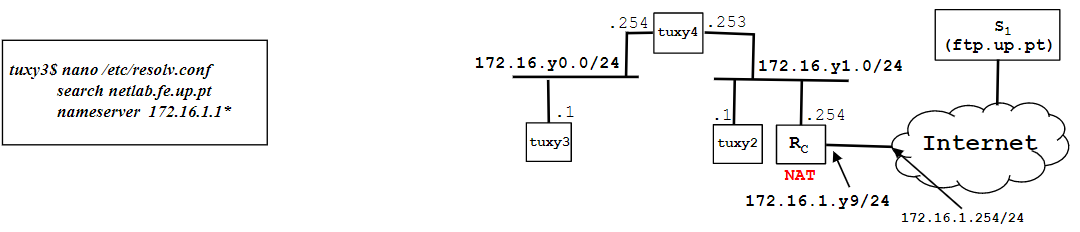
\includegraphics[scale=0.32]{imagens/Exp5.png}
\caption{Arquitetura da Quinta Experiência}
\label{fig:exp5}
\end{figure}

Esta experiência tem como objectivo saber como configurar um serviço DNS numa máquina e descobrir que pacotes são trocados pelo serviço de DNS, para além da informação contida nos mesmos.

Os comandos usados para esta experiência podem ser encontrados no Anexo \ref{exp5_steps}.

\subsubsection{Análise dos Logs}

Esta experiência contém apenas um log (Figura \ref{fig:exp5_logs}) da qual se vão retirar maior parte das conclusões.

Para configurar um serviço de DNS numa máquina só é necessário adicionar uma linha ao ficheiro "etc/resolv.conf" contendo o nome do servidor a usar e o endereço IP do mesmo. Após ter o DNS configurado, aparecerão pacotes relativos ao DNS nos logs.

Ao realizar um ping são enviados 2 pacotes DNS com dois pedidos: Adress Mapping Record (A), para pedir o endereço IPv4 do host e IP Version 6 Address Record (AAAA) para pedir o endereço IPv6. Ambos estes pedidos recebem respostas: Para "ftp.up.pt" o endereço IPv4 é 193.137.29.15 e o endereço IPv6 é 2001:690:2200:1200::15.

Após um ping ser enviado com sucesso e obter resposta, é enviado outro pedido DNS, agora do tipo Reverse-lookup Pointer Record (PTR) para, a partir do endereço IP obtido anteriormente, encontrar todos os host names, que no caso anterior, devolve "mirrors.up.pt". Na figura \ref{fig:exp5_logs} foram feitos pings para "ftp.up.pt" e para "google.com".